\documentclass{ximera}

%\usepackage{todonotes}

\newcommand{\todo}{}

\usepackage{esint} % for \oiint
\ifxake%%https://math.meta.stackexchange.com/questions/9973/how-do-you-render-a-closed-surface-double-integral
\renewcommand{\oiint}{{\large\bigcirc}\kern-1.56em\iint}
\fi


\graphicspath{
  {./}
  {ximeraTutorial/}
  {basicPhilosophy/}
  {functionsOfSeveralVariables/}
  {normalVectors/}
  {lagrangeMultipliers/}
  {vectorFields/}
  {greensTheorem/}
  {shapeOfThingsToCome/}
  {dotProducts/}
  {partialDerivativesAndTheGradientVector/}
  {../productAndQuotientRules/exercises/}
  {../normalVectors/exercisesParametricPlots/}
  {../continuityOfFunctionsOfSeveralVariables/exercises/}
  {../partialDerivativesAndTheGradientVector/exercises/}
  {../directionalDerivativeAndChainRule/exercises/}
  {../commonCoordinates/exercisesCylindricalCoordinates/}
  {../commonCoordinates/exercisesSphericalCoordinates/}
  {../greensTheorem/exercisesCurlAndLineIntegrals/}
  {../greensTheorem/exercisesDivergenceAndLineIntegrals/}
  {../shapeOfThingsToCome/exercisesDivergenceTheorem/}
  {../greensTheorem/}
  {../shapeOfThingsToCome/}
  {../separableDifferentialEquations/exercises/}
  {vectorFields/}
}

\newcommand{\mooculus}{\textsf{\textbf{MOOC}\textnormal{\textsf{ULUS}}}}

\usepackage{tkz-euclide}
\usepackage{tikz}
\usepackage{tikz-cd}
\usetikzlibrary{arrows}
\tikzset{>=stealth,commutative diagrams/.cd,
  arrow style=tikz,diagrams={>=stealth}} %% cool arrow head
\tikzset{shorten <>/.style={ shorten >=#1, shorten <=#1 } } %% allows shorter vectors

\usetikzlibrary{backgrounds} %% for boxes around graphs
\usetikzlibrary{shapes,positioning}  %% Clouds and stars
\usetikzlibrary{matrix} %% for matrix
\usepgfplotslibrary{polar} %% for polar plots
\usepgfplotslibrary{fillbetween} %% to shade area between curves in TikZ
%\usetkzobj{all}
\usepackage[makeroom]{cancel} %% for strike outs
%\usepackage{mathtools} %% for pretty underbrace % Breaks Ximera
%\usepackage{multicol}
\usepackage{pgffor} %% required for integral for loops



%% http://tex.stackexchange.com/questions/66490/drawing-a-tikz-arc-specifying-the-center
%% Draws beach ball
\tikzset{pics/carc/.style args={#1:#2:#3}{code={\draw[pic actions] (#1:#3) arc(#1:#2:#3);}}}



\usepackage{array}
\setlength{\extrarowheight}{+.1cm}
\newdimen\digitwidth
\settowidth\digitwidth{9}
\def\divrule#1#2{
\noalign{\moveright#1\digitwidth
\vbox{\hrule width#2\digitwidth}}}




% \newcommand{\RR}{\mathbb R}
% \newcommand{\R}{\mathbb R}
% \newcommand{\N}{\mathbb N}
% \newcommand{\Z}{\mathbb Z}

\newcommand{\sagemath}{\textsf{SageMath}}


%\renewcommand{\d}{\,d\!}
%\renewcommand{\d}{\mathop{}\!d}
%\newcommand{\dd}[2][]{\frac{\d #1}{\d #2}}
%\newcommand{\pp}[2][]{\frac{\partial #1}{\partial #2}}
% \renewcommand{\l}{\ell}
%\newcommand{\ddx}{\frac{d}{\d x}}

% \newcommand{\zeroOverZero}{\ensuremath{\boldsymbol{\tfrac{0}{0}}}}
%\newcommand{\inftyOverInfty}{\ensuremath{\boldsymbol{\tfrac{\infty}{\infty}}}}
%\newcommand{\zeroOverInfty}{\ensuremath{\boldsymbol{\tfrac{0}{\infty}}}}
%\newcommand{\zeroTimesInfty}{\ensuremath{\small\boldsymbol{0\cdot \infty}}}
%\newcommand{\inftyMinusInfty}{\ensuremath{\small\boldsymbol{\infty - \infty}}}
%\newcommand{\oneToInfty}{\ensuremath{\boldsymbol{1^\infty}}}
%\newcommand{\zeroToZero}{\ensuremath{\boldsymbol{0^0}}}
%\newcommand{\inftyToZero}{\ensuremath{\boldsymbol{\infty^0}}}



% \newcommand{\numOverZero}{\ensuremath{\boldsymbol{\tfrac{\#}{0}}}}
% \newcommand{\dfn}{\textbf}
% \newcommand{\unit}{\,\mathrm}
% \newcommand{\unit}{\mathop{}\!\mathrm}
% \newcommand{\eval}[1]{\bigg[ #1 \bigg]}
% \newcommand{\seq}[1]{\left( #1 \right)}
% \renewcommand{\epsilon}{\varepsilon}
% \renewcommand{\phi}{\varphi}


% \renewcommand{\iff}{\Leftrightarrow}

% \DeclareMathOperator{\arccot}{arccot}
% \DeclareMathOperator{\arcsec}{arcsec}
% \DeclareMathOperator{\arccsc}{arccsc}
% \DeclareMathOperator{\si}{Si}
% \DeclareMathOperator{\scal}{scal}
% \DeclareMathOperator{\sign}{sign}


%% \newcommand{\tightoverset}[2]{% for arrow vec
%%   \mathop{#2}\limits^{\vbox to -.5ex{\kern-0.75ex\hbox{$#1$}\vss}}}
% \newcommand{\arrowvec}[1]{{\overset{\rightharpoonup}{#1}}}
% \renewcommand{\vec}[1]{\arrowvec{\mathbf{#1}}}
% \renewcommand{\vec}[1]{{\overset{\boldsymbol{\rightharpoonup}}{\mathbf{#1}}}}

% \newcommand{\point}[1]{\left(#1\right)} %this allows \vector{ to be changed to \vector{ with a quick find and replace
% \newcommand{\pt}[1]{\mathbf{#1}} %this allows \vec{ to be changed to \vec{ with a quick find and replace
% \newcommand{\Lim}[2]{\lim_{\point{#1} \to \point{#2}}} %Bart, I changed this to point since I want to use it.  It runs through both of the exercise and exerciseE files in limits section, which is why it was in each document to start with.

% \DeclareMathOperator{\proj}{\mathbf{proj}}
% \newcommand{\veci}{{\boldsymbol{\hat{\imath}}}}
% \newcommand{\vecj}{{\boldsymbol{\hat{\jmath}}}}
% \newcommand{\veck}{{\boldsymbol{\hat{k}}}}
% \newcommand{\vecl}{\vec{\boldsymbol{\l}}}
% \newcommand{\uvec}[1]{\mathbf{\hat{#1}}}
% \newcommand{\utan}{\mathbf{\hat{t}}}
% \newcommand{\unormal}{\mathbf{\hat{n}}}
% \newcommand{\ubinormal}{\mathbf{\hat{b}}}

% \newcommand{\dotp}{\bullet}
% \newcommand{\cross}{\boldsymbol\times}
% \newcommand{\grad}{\boldsymbol\nabla}
% \newcommand{\divergence}{\grad\dotp}
% \newcommand{\curl}{\grad\cross}
%\DeclareMathOperator{\divergence}{divergence}
%\DeclareMathOperator{\curl}[1]{\grad\cross #1}
% \newcommand{\lto}{\mathop{\longrightarrow\,}\limits}

% \renewcommand{\bar}{\overline}

\colorlet{textColor}{black}
\colorlet{background}{white}
\colorlet{penColor}{blue!50!black} % Color of a curve in a plot
\colorlet{penColor2}{red!50!black}% Color of a curve in a plot
\colorlet{penColor3}{red!50!blue} % Color of a curve in a plot
\colorlet{penColor4}{green!50!black} % Color of a curve in a plot
\colorlet{penColor5}{orange!80!black} % Color of a curve in a plot
\colorlet{penColor6}{yellow!70!black} % Color of a curve in a plot
\colorlet{fill1}{penColor!20} % Color of fill in a plot
\colorlet{fill2}{penColor2!20} % Color of fill in a plot
\colorlet{fillp}{fill1} % Color of positive area
\colorlet{filln}{penColor2!20} % Color of negative area
\colorlet{fill3}{penColor3!20} % Fill
\colorlet{fill4}{penColor4!20} % Fill
\colorlet{fill5}{penColor5!20} % Fill
\colorlet{gridColor}{gray!50} % Color of grid in a plot

\newcommand{\surfaceColor}{violet}
\newcommand{\surfaceColorTwo}{redyellow}
\newcommand{\sliceColor}{greenyellow}




\pgfmathdeclarefunction{gauss}{2}{% gives gaussian
  \pgfmathparse{1/(#2*sqrt(2*pi))*exp(-((x-#1)^2)/(2*#2^2))}%
}


%%%%%%%%%%%%%
%% Vectors
%%%%%%%%%%%%%

%% Simple horiz vectors
\renewcommand{\vector}[1]{\left\langle #1\right\rangle}


%% %% Complex Horiz Vectors with angle brackets
%% \makeatletter
%% \renewcommand{\vector}[2][ , ]{\left\langle%
%%   \def\nextitem{\def\nextitem{#1}}%
%%   \@for \el:=#2\do{\nextitem\el}\right\rangle%
%% }
%% \makeatother

%% %% Vertical Vectors
%% \def\vector#1{\begin{bmatrix}\vecListA#1,,\end{bmatrix}}
%% \def\vecListA#1,{\if,#1,\else #1\cr \expandafter \vecListA \fi}

%%%%%%%%%%%%%
%% End of vectors
%%%%%%%%%%%%%

%\newcommand{\fullwidth}{}
%\newcommand{\normalwidth}{}



%% makes a snazzy t-chart for evaluating functions
%\newenvironment{tchart}{\rowcolors{2}{}{background!90!textColor}\array}{\endarray}

%%This is to help with formatting on future title pages.
\newenvironment{sectionOutcomes}{}{}



%% Flowchart stuff
%\tikzstyle{startstop} = [rectangle, rounded corners, minimum width=3cm, minimum height=1cm,text centered, draw=black]
%\tikzstyle{question} = [rectangle, minimum width=3cm, minimum height=1cm, text centered, draw=black]
%\tikzstyle{decision} = [trapezium, trapezium left angle=70, trapezium right angle=110, minimum width=3cm, minimum height=1cm, text centered, draw=black]
%\tikzstyle{question} = [rectangle, rounded corners, minimum width=3cm, minimum height=1cm,text centered, draw=black]
%\tikzstyle{process} = [rectangle, minimum width=3cm, minimum height=1cm, text centered, draw=black]
%\tikzstyle{decision} = [trapezium, trapezium left angle=70, trapezium right angle=110, minimum width=3cm, minimum height=1cm, text centered, draw=black]



\author{Lee Wayand}

\begin{document}
\begin{exercise}





\[
f(x) = 
\begin{cases}
  -\frac{x}{2} - 4   & \text{ if } [-8, -2)   \\
  (x+2)(x-3) - 1      & \text{ if } [-2, 4]  \\
  3x-16              & \text{ if } (4,8)
\end{cases}
\]






Graph of $y = f(x)$.



\begin{image}
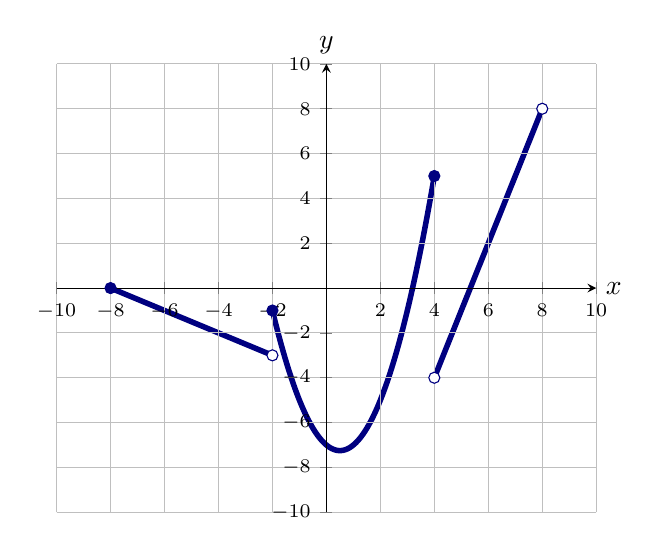
\begin{tikzpicture} 
  \begin{axis}[
            domain=-10:10, ymax=10, xmax=10, ymin=-10, xmin=-10,
            axis lines =center, xlabel=$x$, ylabel=$y$, grid = major,
            ytick={-10,-8,-6,-4,-2,2,4,6,8,10},
            xtick={-10,-8,-6,-4,-2,2,4,6,8,10},
            ticklabel style={font=\scriptsize},
            every axis y label/.style={at=(current axis.above origin),anchor=south},
            every axis x label/.style={at=(current axis.right of origin),anchor=west},
            axis on top
          ]
          
          \addplot [line width=2, penColor, smooth,samples=100,domain=(-8:-2)] {-0.5*x-4};
       	  \addplot [line width=2, penColor, smooth,samples=100,domain=(-2:4)] {(x+2)*(x-3)-1};
       		\addplot [line width=2, penColor, smooth,samples=100,domain=(4:8)] {3*x-16};




			\addplot[color=penColor,fill=penColor,only marks,mark=*] coordinates{(-8,0)};

			\addplot[color=penColor,fill=penColor,only marks,mark=*] coordinates{(-2,-1)};
			\addplot[color=penColor,fill=white,only marks,mark=*] coordinates{(-2,-3)};

			\addplot[color=penColor,fill=penColor,only marks,mark=*] coordinates{(4,5)};
			\addplot[color=penColor,fill=white,only marks,mark=*] coordinates{(4,-4)};

			\addplot[color=penColor,fill=white,only marks,mark=*] coordinates{(8,8)};

  \end{axis}
\end{tikzpicture}
\end{image}







\begin{question} Domain


The domain is given in the definition of the function.

\[
\left[ \answer{-8}, \answer{-2} \right) \cup \left[  \answer{-2}, \answer{4} \right] \cup \left(  \answer{4}, \answer{8} \right) = \left[ \answer{-8}, \answer{8} \right)
\]


\end{question}







\begin{question} Continuity


The three pieces in the definition of $f(x)$ are linear, quadratic, and linear.  These are continuous functions.  Therefore, the only candidates for discontinuities or singularities are the endpoints of the defining intervals.

$-8$ is included in $[-8, -2)$ and $-\frac{x}{2} - 4$ is continuous on this interval. \\

$-2$ is a discontinuity of $f$.  Let $d = 1$. For any small $\epsilon > 0$, the interval $(-2 - \epsilon, -2)$ always contains the number $-2 - \frac{\epsilon}{2}$.  


\[
f\left( -2 - \frac{\epsilon}{2} \right) = 1 + \frac{\epsilon}{4} - 4 =  \frac{\epsilon}{4} - 3
\]


\[
f(-2) - f\left( -2 - \frac{\epsilon}{2} \right) = -1 - \frac{\epsilon}{4} + 3 = 2 - \frac{\epsilon}{4} > 1 = d
\]


Every small open interval around $-2$ contains a domain number where the value of $f$ is more than 1 away from $f(-2)$.





Similarly, $4$ is also a discontinuity.  \\



$8$ is not in the domain.  It cannot be a singularity since it is not a hole in the domain.  For the number $a$ to be a hole, there would need to be an open interval inside the domain, except for $a$:  $(c, a) \cup (a, b)$. 


\end{question}





\begin{question} Zeros


The defininng pieces of $f$ have zeros.  The linear pieces have one zero and the quadratic piece has two zeros.  We'll determine these zeros and then see if they are in the domain of $f$. \\



The zero of $f_1(x) = -\frac{x}{2} - 4$ is $\answer{-8}$, which is included in the domain of $f$. \\

There are two zeros for $f_2(x) = (x+2)(x-3) - 1$. \\


$ 0 = (x+2)(x-3) - 1 = x^2 - x - 7$ \\

\[
x = \frac{1 \pm \sqrt{(-1)^2 - 4 \cdot 1 \cdot (-7)}}{2} = \frac{1 \pm \sqrt{29}}{2}
\]


Only $\answer{\frac{1 - \sqrt{29}}{2}}$ is contained in the domain of $f$. \\


The zero of $f_3(x) = 3x-16$ is $\answer{\frac{16}{3}}$, which is included in the domain of $f$. \\




$f$ has three zeros:  $-8, \frac{1 \pm \sqrt{29}}{2}, \frac{16}{3}$.


\end{question}





\begin{question} End-Behavior



End-behavior is explicitly for unbounded domains.  Therefore, there is no end-behavior for $f$.


\end{question}






\begin{question} Behavior



From the graph, we can see that $f$ decreases, then decreases, then increases, then increases.  We want algebraic and functional reasoning. $iRoC_f(x)$ will give us behavior information.   \\


Avoiding both discontinuities, we have

\[
iRoC_f(x) = 
\begin{cases}
  -\frac{1}{2}   & \text{ if } [-8, -2)   \\
  2x - 1      & \text{ if } (-2, 4)  \\
  3             & \text{ if } (4,8)
\end{cases}
\]


On $[-8, -2)$, $f$ is a linear function with a negative rate of change, or we have $iRoC_f(x) = -\frac{1}{2}$, which is always negative.  Both of these tell us that $f$ is decreasing on $[-8, -2)$. \\


On $(-2, 4)$, $f$ is a quadratic function.  $iRoC_f(x) = 0$ when $2x - 1 = 0$, which gives us $x = \frac{1}{2}$.


\begin{itemize}
\item $2x - 1 \wordChoice{\choice[correct]{<} \choice{>}}  0$ on  $\left( -2, \frac{1}{2}  \right)$ where $f$ is decreasing.
\item $2x - 1 \wordChoice{\choice{<} \choice[correct]{>}}  0$ on  $\left( \frac{1}{2}, 4 \right)$ where $f$ is increasing.
\end{itemize}

On $(4, 8)$, $f$ is a linear function with a positive rate of change, or we have $iRoC_f(x) = 3$, which is always positive.  Both of these tell us that $f$ is increasing on $(4, 8)$. \\




$\blacktriangleright$ \textbf{Discontinuities} \\


Both discontinuities are connected to the middle piece of the function (the parabola). The critical number for the quadratic can be included in both pieces.



\begin{itemize}
\item $f$ decreases on $[-8, -2)$
\item $f$ decreases on $\left[ -2, \frac{1}{2}  \right]$
\item $f$ decreases on $\left[ \frac{1}{2}, 4 \right)$
\item $f$ decreases on $(4, 8)$
\end{itemize}

\begin{warning}


$f$ decreases on $[-8, -2)$ and on $\left[ -2, \frac{1}{2}  \right]$, however, $f$ does not decrease on the union $[-8, -2) \cup \left[ -2, \frac{1}{2}  \right]$.

We can easily see this in the graph, because the graph jumps up to the right at $-2$. \\

We can show this algebraically, by providing a counterexample to the definition of decreasing. Select two domain numbers $a < b$, yet $f(a) < f(b)$.  Our two numbers will be $-2.1 < -2$.


$f(-2.1) = 1.05 - 4 = -2.95 < -1 = f(-2)$


\end{warning}


\end{question}





\begin{question} Global Maximum






The graph suggests that there is no global maximum. Algebraically, we can establish this by showing that 

\begin{itemize}
\item $f \leq 5$ on $[-8, 4]$ 
\item $f$ is continuous and increasing on $(4, 8)$
\end{itemize}

We already have shown the second part. \\



On $[-8, -2)$, $f$ is continuous and decreasing, therefore $f(x) \leq f(-8) = 0 \leq 5$.  \\


On $[-2, 4]$, $f$ is continuous and decreasing and then increasing, therefore $f(x)$ is less than or equal to the maximum of the endpoint values. $f(-2) = -1$ and $f(4) = 5$. \\


On $(4, 8)$ $f$ is continuous and \wordChoice{\choice[correct]{increasing} \choice{decreasing}} , therefore, since $8 \notin (4, 8)$, there is no maximum value.



\begin{idea} Open Interval

To see that $f$ has no maximum value on $(4, 8)$, pretend there is a maximum value. \\


Suppose $c \in (4, 8)$ with $f(x) \leq f(c)$ for all $x \in (4, 8)$.


Then, since $(4, 8)$ is an open interval we know that $\frac{c+8}{2} \in (4, 8)$ and $f\left( \frac{c+8}{2} \right) > f(c)$, because $f$ is increasing and $\frac{c+8}{2} > c$.







\end{idea}


\end{question}

\begin{warning}


Yes, it is easier to say that the graph shows us there is no maximum.  However, we have already seen graphs which have been misleading. We cannot trust the visual information from graphs to be proof.  We don't trust graphs that much.  Algebra and function reasoning is the only things we trust to be exact and to cover all posibilities.

\end{warning}






\begin{question} Global Minimum 


Yes, the graph convinces us that there is a global minimum and it is connected to the vertex of the parabola. \\


Now, we let that direct our algebra.  Here is our plan (which you can carry out):


\begin{enumerate}
\item On $[-8, -2)$, $f$ is decreasing, so $f$ is greater than $-\frac{-2}{2} - 4$.
\item On $(-2, 4)$, $f$ is a quadratic with a positive leading coefficient.  That means a minimum at the critical number, which is included in the domain.
\item On $(4, 8)$, $f$ is increasing, so $f$ is greater than $3 \cdot 4 - 16$.
\end{enumerate}

That will establish $f\left( \frac{1}{2} \right) = -\frac{29}{4}$ as the global minimum.

\end{question}










\begin{question} Local Maximums 

$-2$ and $4$ are locations of local maximums.  We'll explain $4$. \\


First, we need an open interval around $4$.  We'll chose $\left( 4-\frac{1}{2}, 4 + \frac{1}{2} \right)$.


On $\left( 4-\frac{1}{2}, 4 \right]$, $f$ is increasing, which means $f(x) \leq f(4) = 5$. \\

On $\left( 4, 4 + \frac{1}{2} \right]$, $f$ is increasing, which means $f(x) \leq f\left( 4 + \frac{1}{2} \right) = -2.5 < f(4) = 5$


$f(x) \leq f(4)$  for all $x \in \left( 4-\frac{1}{2}, 4 + \frac{1}{2} \right)$.

$f(4)$ is a local maximum.



\end{question}




\begin{question} Range 


We can take the union of the ranges of each of the three pieces.\\


\[
(-3, 0] \cup \left[ -\frac{29}{4}, 5 \right] \cup (-4, 8) = \left[ -\frac{29}{4}, 8 \right)
\]


\end{question}





\end{exercise}
\end{document}